\documentclass{article}
\usepackage[utf8]{inputenc}
\parskip = 0.75em
\parindent = 10mm
\def\baselinestretch{1}
\usepackage {float}
\usepackage{listings}
\usepackage{subcaption}
\usepackage[usenames]{color}
\usepackage[numbers,sort&compress]{natbib}
\usepackage{multirow, array}
\usepackage[spanish]{babel}
	\deactivatetilden
	\spanishdecimal{.}
	\addto\captionsspanish{\def\tablename{Tabla}}
	\addto\captionsspanish{\def\listtablename{\'Indice de tablas}}

\usepackage{amsmath,amsfonts,amssymb}
	\allowdisplaybreaks[4]
\usepackage{graphicx}
	\graphicspath{{Figuras/}}
\usepackage[clearempty,pagestyles]{titlesec}
\usepackage{anysize}

\def\baselinestretch{1.5}
\papersize{27.9cm}{21.5cm} 
\marginsize{2cm}{2cm}{1cm}{1cm}

\begin{document}


	\begin{center}
	\huge{\textbf{Tarea 9 Interacciones entre partículas}}\\
	
	\textsc{ \Large Susana Ruiz Nuñez}
	\end{center}


\section{Planteamiento del problema} 
En esta práctica \cite{satu} se trabajan los fenómenos de atracción y repulsión entre partículas. Se tienen \textit{n} partículas que habitan en un cuadro unitario bidimensional y cada partícula tiene una carga eléctrica, distribuida entre $[-1,1]$ donde cargas de un mismo signo producirán repulsión y cargas opuestas atracción. La magnitud de la fuerza será proporcional a la diferencia de magnitud de las cargas (mayores diferencias resultando en fuerzas mayores), y además la fuerza será inversamente proporcional a la distancia euclideana entre las partículas. Se pide agregar una \textit{masa} a cada partícula que cause fuerzas gravitacionales y estudiar la distribución de velocidades de las partículas
y verificar la relación entre los factores: velocidad, magnitud de la carga y masa de las partículas.

\section{Metodología}
En el modelo base \cite{satu} se tienen ya implementadas la atracción y repulsión entre partículas y las sumas de los efectos de todas las fuerzas individuales existentes hasta el momento. Este proyecto se realiza con Python 3.8 y fue necesario reestructurar lo que el multiprocessing estaba haciendo en el código \cite{vict}. Lo primero que se hizo fue agregar una masa \textit{m} de cinco diferentes tamaños. Posteriormente se agrega la constante gravitacional \textit{G} que creará otra fuerza de atracción entre las partículas a parte de la ya existente. Dicha fuerza se obtiene siguiendo la ley de Newton de la fuerza gravitacional donde plantea que toda partícula en el universo atrae a cualquier otra partícula con una fuerza que es directamente proporcional al producto de sus masas e inversamente proporcional al cuadrado de la distancia entre ellas.


\section{Resultados}
Los resultados obtenidos muestran una variación considerable en las velocidades cuando se le agrega la masa ya que actúan las fuerzas gravitacionales sobre ella y la diferencia de cuando las partículas no tienen masa. Por supuesto se observa que para cuando las partículas no tienen masa las velocidades que alcanzan son mucho mayores que cuando tienen una fuerza gravitacional incluida.


\begin{figure}
\centering
	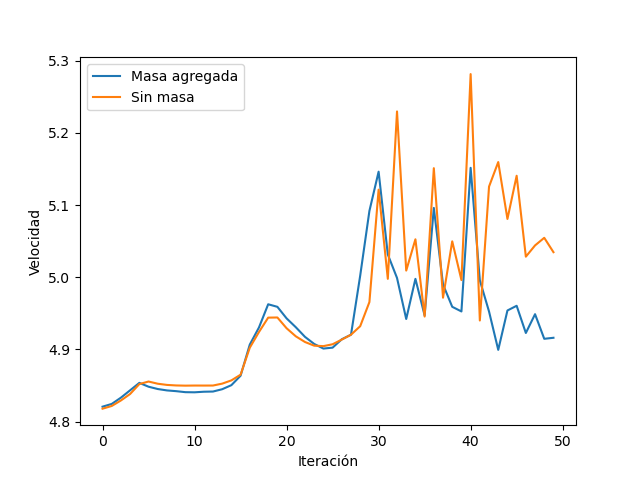
\includegraphics[width=\linewidth]{Figure_1.png}
	\caption{Comportamiento de las velocidades de las partículas con masa agregada y sin masa para 50 iteraciones.}
	\label{1}		
\end{figure}
\section{Conclusiones}
Se concluye que los experimentos realizados cumplen con las leyes de la física correctamente, al tener una variación cuando se le agrega una masa y una fuerza gravitacional a las partículas (comportamiento que se asemeja a lo que ocurre en los sucesos de la vida real).

\bibliography{Tarea9}
\bibliographystyle{plainnat}
\end{document} 
